\let\negmedspace\undefined
\let\negthickspace\undefined
\documentclass[journal]{IEEEtran}
\usepackage[a5paper, margin=10mm, onecolumn]{geometry}
%\usepackage{lmodern} % Ensure lmodern is loaded for pdflatex
\usepackage{tfrupee} % Include tfrupee package

\setlength{\headheight}{1cm} % Set the height of the header box
\setlength{\headsep}{0mm}     % Set the distance between the header box and the top of the text

\usepackage{gvv-book}
\usepackage{gvv}
\usepackage{cite}
\usepackage{amsmath,amssymb,amsfonts,amsthm,mathtools}
\usepackage{algorithmic}
\usepackage{graphicx}
\usepackage{textcomp}
\usepackage{xcolor}
\usepackage{txfonts}
\usepackage{listings}
\usepackage{enumitem}
\usepackage{mathtools}
\usepackage{gensymb}
\usepackage{comment}
\usepackage[breaklinks=true]{hyperref}
\usepackage{tkz-euclide} 
\usepackage{listings}
\def\inputGnumericTable{}                                 
\usepackage[latin1]{inputenc}                                
\usepackage{color}                                            
\usepackage{array}                                            
\usepackage{longtable}                                       
\usepackage{calc}                                             
\usepackage{multirow}                                         
\usepackage{hhline}                                           
\usepackage{ifthen}                                           
\usepackage{lscape}
\begin{document}

\bibliographystyle{IEEEtran}
\vspace{3cm}

\title{1.10.30}
\author{EE24BTECH11002 - Agamjot Singh
}
% \maketitle
% \newpage
% \bigskip
{\let\newpage\relax\maketitle}

\renewcommand{\thefigure}{\theenumi}
\renewcommand{\thetable}{\theenumi}
\setlength{\intextsep}{10pt} % Space between text and floats

\textbf{Question:}
\newline
If a line has direction ratios 2, -1, 2, determine its direction cosines.
\newline
\textbf{Solution:}
\newline
Let 
\begin{align}
	\vec{A} &= \myvec{2\\-1\\2}\\
	\norm{A} &= \sqrt{\vec{A}\top\vec{A}}\\
		     &= \sqrt{\myvec{2 & -1 & 2}\myvec{2\\-1\\2}}\\
	\implies \norm{A} &= 3
\end{align}
The unit direction vector of the line is
\begin{align}
	\frac{\vec{A}}{\norm{\vec{A}}} = \frac{\myvec{2\\-1\\2}}{3} = \myvec{\frac{2}{3}\\\frac{-1}{3}\\\frac{2}{3}}
\end{align}
Hence, the direction cosines of the line are $\frac{2}{3}$, $\frac{-1}{3}$ and $\frac{2}{3}$.

\begin{figure}[h!]
   \centering
   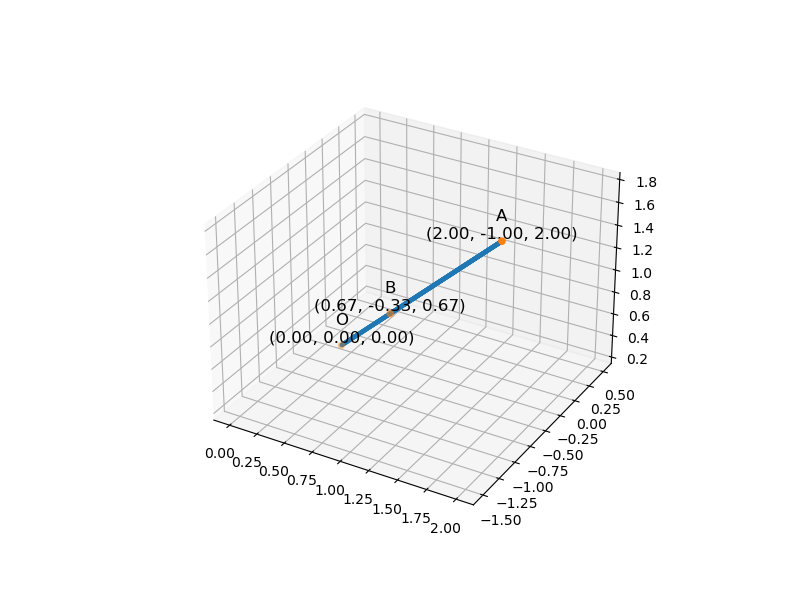
\includegraphics[width=0.7\linewidth]{figs/graph.png}
   \caption{Line with given direction ratios, where $\vec{B}$ is unit direction vector}
\end{figure}

\end{document}
